\documentclass[a4paper,12pt]{article}
\usepackage[utf8]{inputenc}
\usepackage{listings}
\usepackage{amsmath, amssymb}
\usepackage{geometry}
\usepackage{booktabs}
\usepackage{graphicx}


\geometry{left=2.5cm, right=2.5cm, top=2.5cm, bottom=2.5cm}
\usepackage{fancyhdr}
\pagestyle{fancy}
\fancyhf{}
\lhead{Lösung zur Algorithmusanalyse}
\cfoot{\thepage}

\begin{document}
	
	\title{\textbf{Musterlösungen}}
	\date{\today}
	\maketitle
	
	\section*{Lösung zu Aufgabe 1: Analyse eines Algorithmus}
	\section*{Gegebener Java-Code}
	
	\begin{verbatim}
		public class Algorithmus {
			public static int berechne(int x, int y) {
				if (y == 0) {
					return x;
				}
				return berechne(y, x % y);
			}
			
			public static void main(String[] args) {
				int wert1 = 56;
				int wert2 = 98;
				System.out.println("Ergebnis: " + berechne(wert1, wert2));
			}
		}
	\end{verbatim}
	
	\section*{1. Beschreibung der Funktionsweise}
	
	Der Algorithmus berechnet den \textbf{größten gemeinsamen Teiler (ggT)} zweier Zahlen mithilfe des \textbf{Euklidischen Algorithmus}. Die Rekursion basiert auf der Formel:
	\[ ggT(a, b) = \begin{cases} a, & \text{wenn } b = 0 \\ ggT(b, a\mod b), & \text{sonst} \end{cases} \]
	
	\section*{2. Art der Implementierung und Vorteile}
	
	\textbf{Implementierung:} Der Algorithmus verwendet eine \textbf{rekursive Methode}. Vorteile sind:
	\begin{itemize}
		\item Elegante und kompakte Umsetzung
		\item Effizient für große Zahlen
		\item Direkte Umsetzung der mathematischen Definition
	\end{itemize}
	
	\section*{3. Beispielrechnung für berechne(56, 98)}
	
	\begin{align*}
		\text{berechne}(56, 98) & \to \text{berechne}(98, 56) \\
		\text{berechne}(98, 56) & \to \text{berechne}(56, 42) \\
		\text{berechne}(56, 42) & \to \text{berechne}(42, 14) \\
		\text{berechne}(42, 14) & \to \text{berechne}(14, 0) \\
		\text{Ergebnis: } & 14
	\end{align*}
	
	\section*{4. Anzahl der Aufrufe}
	
	Insgesamt werden \textbf{4 rekursive Aufrufe} benötigt, um den ggT zu berechnen.
	
	\section*{5. Herleitung der Zeitkomplexität}
	
	Die Anzahl der Rekursionsschritte im Euklidischen Algorithmus hängt davon ab, wie schnell sich die Werte \( x \) und \( y \) durch die Modulo-Operation verringern. Eine grundlegende Eigenschaft dieses Algorithmus ist:
	
	\[ a_{i+1} = a_i \mod a_{i-1} \]
	
	Ein wichtiger mathematischer Zusammenhang wurde von Gabriel Lamé (1812) bewiesen: Die Anzahl der Rekursionsschritte ist höchstens proportional zur Anzahl der Fibonacci-Zahlen, die in \( x \) und \( y \) enthalten sind.
	
	Sei \( F_n \) die \( n \)-te Fibonacci-Zahl. Falls \( x \) und \( y \) zwei aufeinanderfolgende Fibonacci-Zahlen sind, dann ist die maximale Anzahl der Rekursionsschritte \( O(n) \), wobei gilt:
	
	\[ F_n \approx \frac{\varphi^n}{\sqrt{5}}, \quad \text{mit } \varphi = \frac{1 + \sqrt{5}}{2} \approx 1.618. \]
	
	Daher folgt:
	
	\[ n = O(\log \min(x, y)). \]
	
	Das bedeutet, dass der Euklidische Algorithmus in maximal \( O(\log \min(x, y)) \) Schritten terminiert.
	
	\subsection*{Beispiel 1: ggT(56, 98)}
	
	Die Berechnungsschritte sind:
	\begin{align*}
		ggT(56, 98) &\to ggT(98, 56) \\
		ggT(98, 56) &\to ggT(56, 42) \\
		ggT(56, 42) &\to ggT(42, 14) \\
		ggT(42, 14) &\to ggT(14, 0) \\
		\text{Ergebnis: } &14
	\end{align*}
	
	Hier sehen wir, dass in jedem Schritt die kleinere Zahl stark reduziert wird, insbesondere durch die Modulo-Operation.
	
	\subsection*{Beispiel 2: ggT(89, 55)}
	
	Die Zahlen 89 und 55 gehören zur Fibonacci-Folge. Der Euklidische Algorithmus benötigt bei Fibonacci-Zahlen die meisten Schritte:
	\begin{align*}
		ggT(89, 55) &\to ggT(55, 34) \\
		ggT(55, 34) &\to ggT(34, 21) \\
		ggT(34, 21) &\to ggT(21, 13) \\
		ggT(21, 13) &\to ggT(13, 8) \\
		ggT(13, 8) &\to ggT(8, 5) \\
		ggT(8, 5) &\to ggT(5, 3) \\
		ggT(5, 3) &\to ggT(3, 2) \\
		ggT(3, 2) &\to ggT(2, 1) \\
		ggT(2, 1) &\to ggT(1, 0) \\
		\text{Ergebnis: } &1
	\end{align*}
	
	Wir haben hier \textbf{9 Schritte} benötigt. Tatsächlich wächst die Anzahl der Schritte proportional zur Anzahl der Stellen in der Binärdarstellung von 89, was der logarithmischen Zeitkomplexität entspricht.
	
	\textbf{Zusammenfassung:} Die Anzahl der Schritte entspricht ungefähr der Anzahl der Male, die man eine Zahl halbieren kann, bevor sie 1 erreicht. Das ist genau der logarithmische Zusammenhang, weshalb der Algorithmus in \( O(\log \min(x, y)) \) Schritten terminiert.
	\subsection*{Logarithmus-Basen und Big-\( \mathcal{O} \): Warum die Basis egal ist?}
	
	\textbf{1. Unterschied bei konkreten Werten:}
	
	Die Basis eines Logarithmus verändert den Zahlenwert:
	
	\begin{align*}
		\log_{10}(55) &\approx 1{,}74 \\
		\ln(55) &\approx 4{,}007 \\
		\log_\varphi(55) &\approx 8{,}33 \quad \text{mit } \varphi = \frac{1 + \sqrt{5}}{2} \approx 1{,}618
	\end{align*}
	
	Diese Werte unterscheiden sich, weil jede Basis anders "zählt".
	
	\vspace{1em}
	\textbf{2. Umrechnung zwischen Basen:}
	
	Für beliebige Basen \( b \) und \( k \) gilt:
	
	\[
	\log_b(n) = \frac{\log_k(n)}{\log_k(b)} = \text{Konstante} \cdot \log_k(n)
	\]
	
	→ Der Unterschied ist nur ein \textbf{konstanter Faktor}.
	
	\vspace{1em}
	\textbf{3. Bedeutung für die Big-\( \mathcal{O} \)-Notation:}
	
	In der asymptotischen Laufzeitanalyse (Big-O) ignorieren wir konstante Faktoren:
	
	\[
	O(\log_{10} n) = O(\ln n) = O(\log_\varphi n) = O(\log n)
	\]
	
	→ Die Basis ist asymptotisch \textbf{nicht relevant}.
	
	\vspace{1em}
	\textbf{Fazit:}  
	Bei konkreten Rechnungen macht die Basis des Logarithmus einen Unterschied,  
	aber bei der asymptotischen Betrachtung in der Big-\( \mathcal{O} \)-Notation zählt nur das \emph{Wachstumsverhalten}, nicht die Skala.
	\begin{figure}[h!]
		\centering
		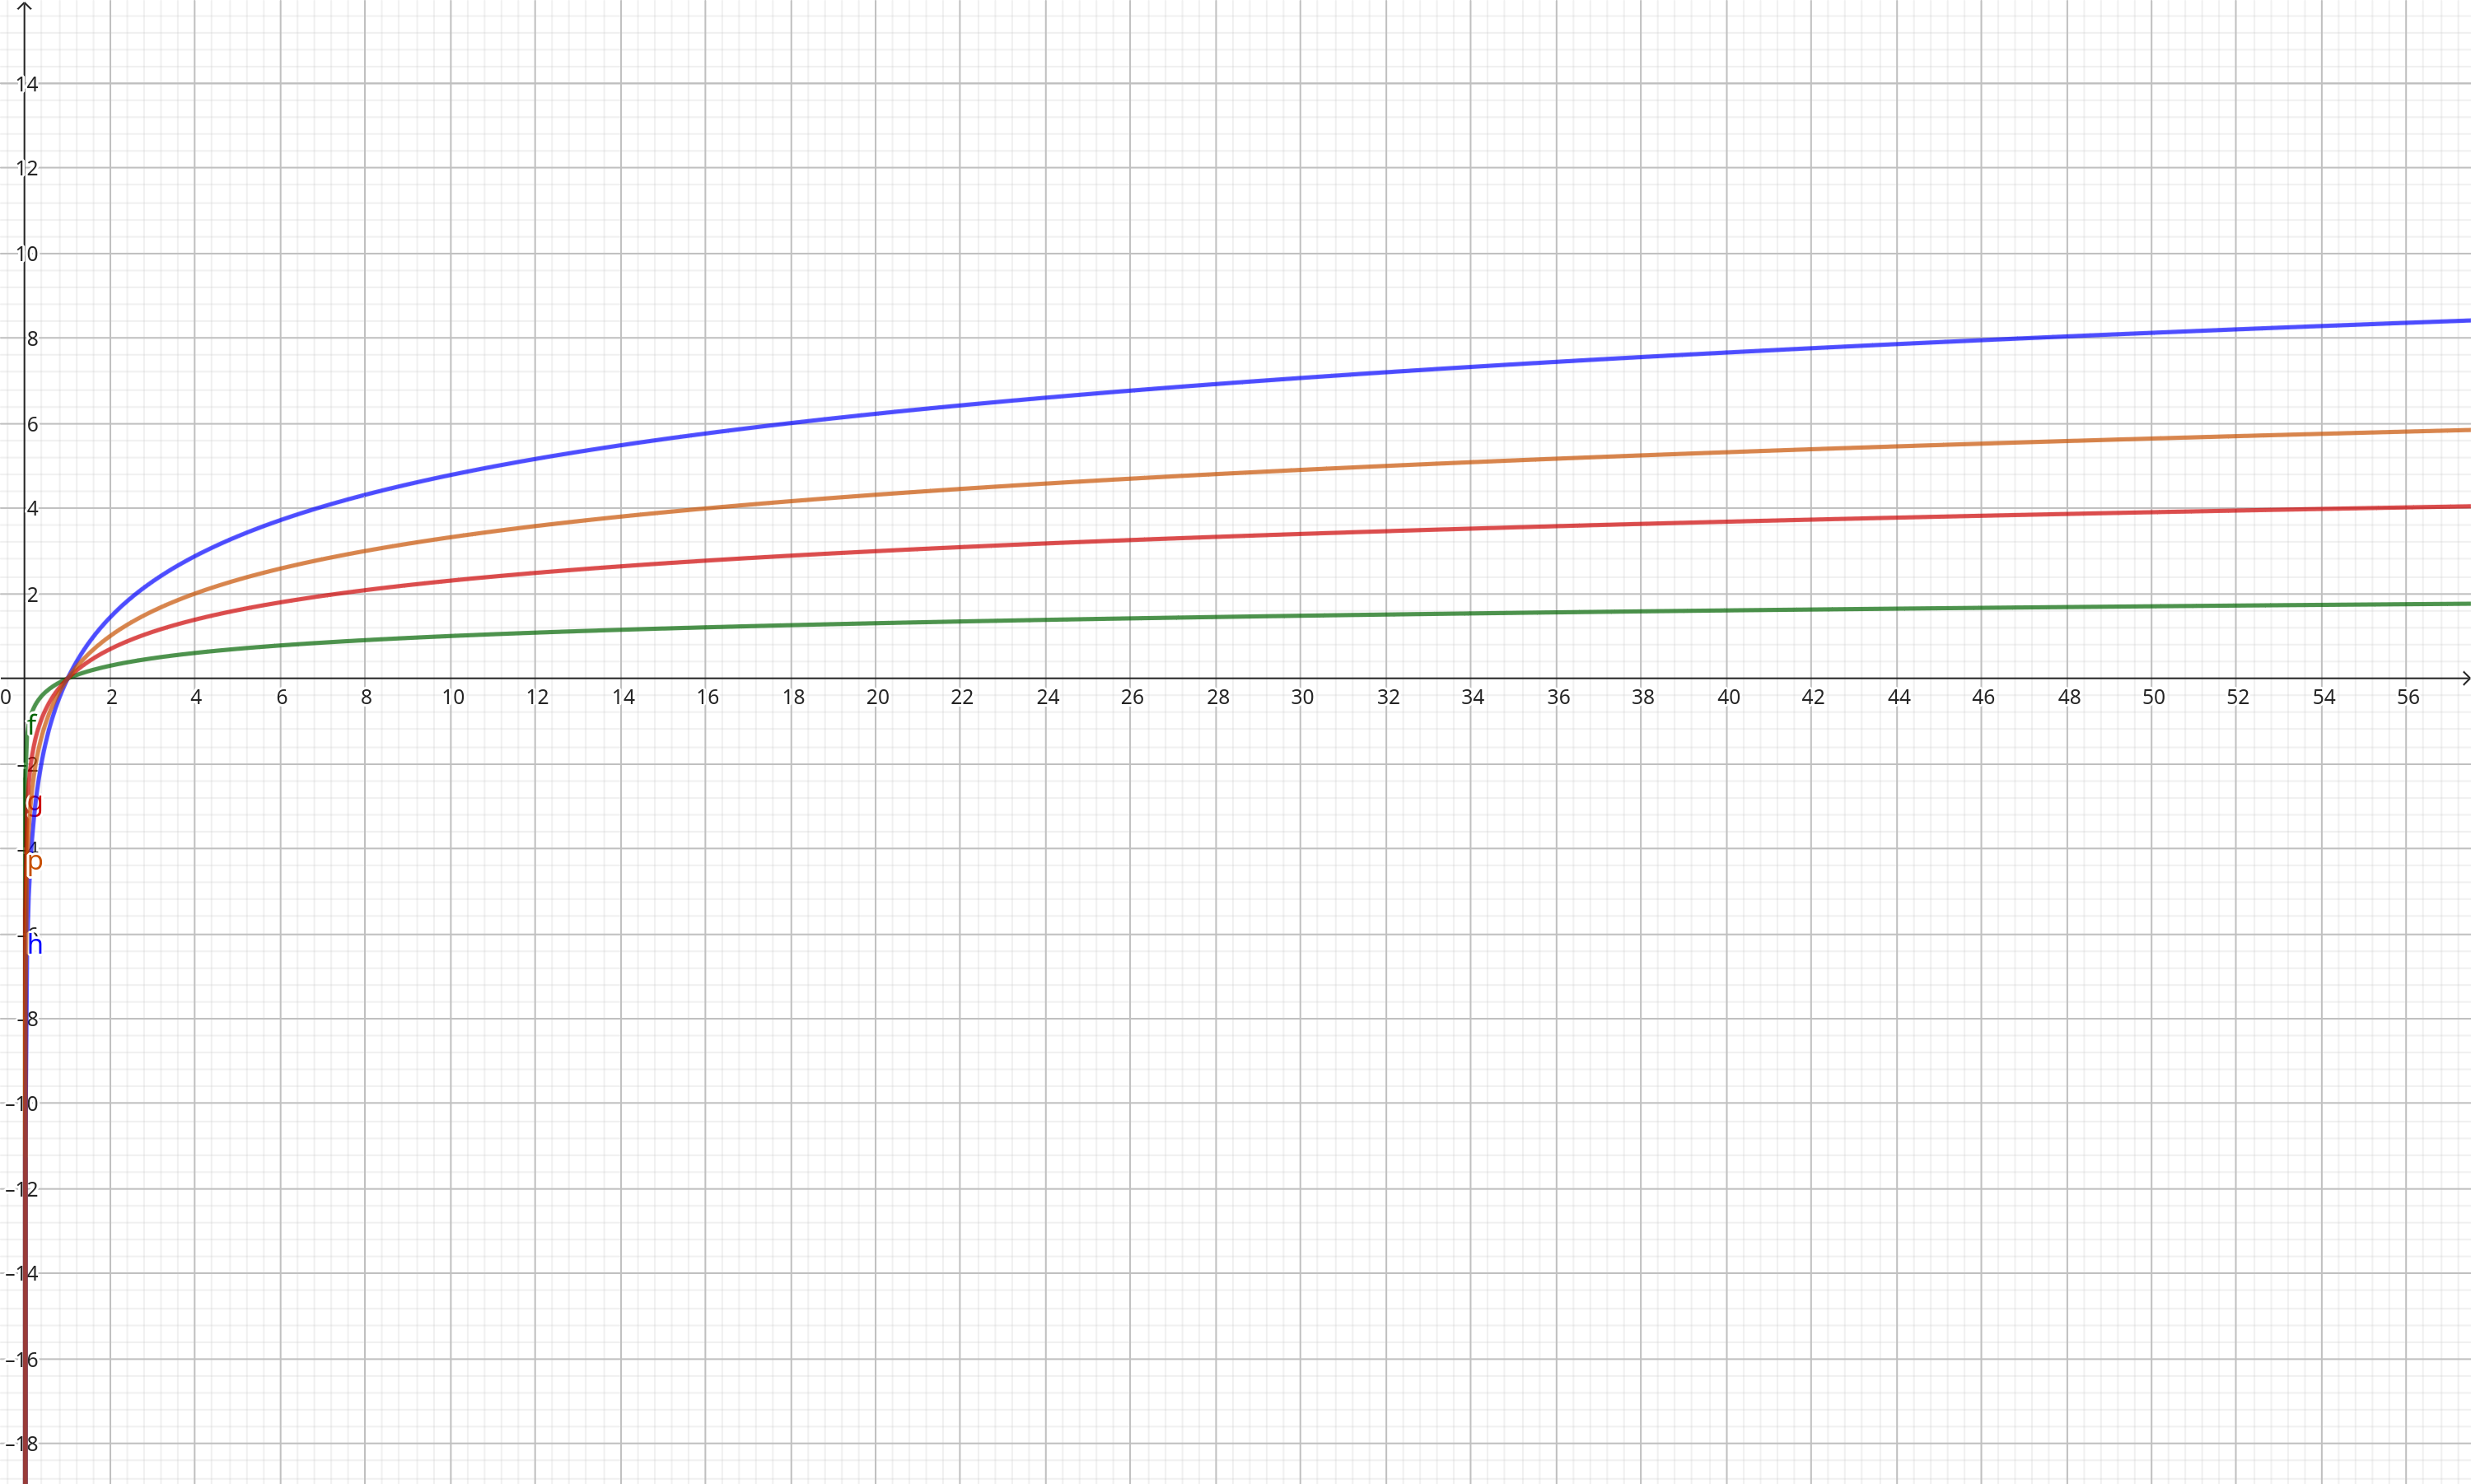
\includegraphics[width=0.75\textwidth]{geogebra-export.png}
		\caption{Vergleich verschiedener Logarithmusfunktionen: \(\log_{10}(n)\), \(\ln(n)\), \(\log_{2}(n)\), \(\log_{\varphi}(n)\)}
		\label{fig:log-vergleich}
	\end{figure}
	
	\subsection*{Warum taucht beim ggT-Algorithmus die goldene Zahl \( \varphi \) auf?}
	
	\textbf{Hintergrund:}  
	Der euklidische Algorithmus zur Berechnung des größten gemeinsamen Teilers (ggT) hat im schlimmsten Fall eine Laufzeit von \( O(\log n) \).  
	Der Worst Case tritt auf, wenn die Eingabezahlen zwei aufeinanderfolgende Fibonacci-Zahlen sind.
	
	\vspace{1em}
	\textbf{1. Fibonacci-Zahlen und der ggT-Algorithmus}
	
	Berechnet man \texttt{ggT(F\textsubscript{n+1}, F\textsubscript{n})}, ergibt jeder Modulo-Schritt das nächste Fibonacci-Glied:
	
	\[
	F_{n+1} \bmod F_n = F_{n-1},\quad
	F_n \bmod F_{n-1} = F_{n-2},\quad \dots,\quad
	F_2 \bmod F_1 = F_0 = 0
	\]
	
	\(\Rightarrow\) Der Algorithmus braucht genau \( n \) Schritte.
	
	\vspace{1em}
	\textbf{2. Wachstum der Fibonacci-Zahlen}
	
	Die Fibonacci-Zahlen wachsen exponentiell nach der Binet-Formel:
	
	\[
	F_n = \frac{\varphi^n - \psi^n}{\sqrt{5}}, \quad
	\text{mit } \varphi = \frac{1 + \sqrt{5}}{2} \approx 1{,}618,\quad
	\psi = \frac{1 - \sqrt{5}}{2}
	\]
	
	Für große \( n \) ist \( \psi^n \) vernachlässigbar, daher:
	
	\[
	F_n \approx \frac{\varphi^n}{\sqrt{5}}
	\quad \Rightarrow \quad
	n \approx \log_\varphi(F_n)
	\]
	
	\vspace{1em}
	\textbf{3. Laufzeitabschätzung:}
	
	Ist \( b = \min(a, b) \), dann:
	
	\[
	T(a, b) \in \Theta(\log_\varphi b) \Rightarrow O(\log b)
	\]
	
	Die Basis \( \varphi \) ergibt sich direkt aus dem Wachstum der Fibonacci-Folge.
	
	\vspace{1em}
	\textbf{4. Fazit:}  
	Die goldene Zahl \( \varphi \) taucht auf, weil Fibonacci-Zahlen den Worst Case im ggT-Algorithmus erzeugen  
	– und diese wachsen mit Basis \( \varphi \). Deshalb ist die Anzahl der Schritte asymptotisch:
	
	\[
	\boxed{O(\log n)}
	\]
	
	wobei die genaue Zahl der Schritte \( \approx \log_\varphi(\min(a, b)) \) ist.
	
	
	
	\section*{6. Vergleich mit iterativen Methoden}
	
	Eine iterative Implementierung vermeidet die Stack-Tiefe der Rekursion und spart Speicher:
	
	\begin{verbatim}
		public class Algorithmus {
			public static int berechne(int x, int y) {
				while (y != 0) {
					int temp = y;
					y = x % y;
					x = temp;
				}
				return x;
			}
		}
	\end{verbatim}
	
	Beide Varianten haben dieselbe Zeitkomplexität \( O(\log \min(x, y)) \), doch die iterative Variante benötigt weniger Speicher.
	
	\section*{Fazit}
	
	- Der Algorithmus berechnet den \textbf{größten gemeinsamen Teiler} zweier Zahlen effizient.
	- Die Rekursion reduziert die Zahlen in jedem Schritt.
	- Die Zeitkomplexität beträgt \( O(\log \min(x, y)) \), was sehr effizient ist.
	- Die mathematische Herleitung basiert auf Fibonacci-Zahlen und der goldenen Zahl \( \varphi \).
	- Eine \textbf{iterative Variante} vermeidet die Tiefe der Rekursion und spart Speicher.
	
	
	\section*{Lösung zu Aufgabe 2: Datenmodellierung und Normalisierung}
	
	\begin{enumerate}
		\item \textbf{Redundanzen in der Tabelle:}
		\begin{itemize}
			\item \textbf{Kundendaten} (Kundenname, Adresse) werden mehrfach gespeichert, wenn ein Kunde mehrere Bestellungen tätigt.
			\item \textbf{Produktdaten} (Produktname, Kategorie, Preis) werden mehrfach gespeichert, wenn dasselbe Produkt mehrfach bestellt wird.
			\item Diese Wiederholungen führen zu \textbf{Redundanz}, \textbf{Speicherplatzverschwendung} und möglichen \textbf{Inkonsistenzen} (z.\,B. bei Änderungen).
		\end{itemize}
		
		\item \textbf{Normalisierung bis zur 3. Normalform:}
		
		\textbf{Ausgangstabelle (nicht normalisiert):}
		
\begin{center}
	\resizebox{\textwidth}{!}{
		\begin{tabular}{|c|c|c|c|c|c|c|c|c|}
			\hline
			BestellID & KundenID & Kundenname & Adresse & ProduktID & Produktname & Kategorie & Preis & Menge \\
			\hline
			1 & 1001 & Anna Müller & Hauptstr. 12, Berlin & 501 & Laptop & Elektronik & 1200 & 1 \\
			2 & 1002 & Thomas Becker & Marktstr. 5, Hamburg & 502 & Smartphone & Elektronik & 800 & 2 \\
			3 & 1001 & Anna Müller & Hauptstr. 12, Berlin & 503 & Drucker & Bürobedarf & 150 & 1 \\
			4 & 1003 & Julia Schmitt & Lindenallee 9, München & 504 & Schreibtisch & Möbel & 300 & 1 \\
			5 & 1002 & Thomas Becker & Marktstr. 5, Hamburg & 505 & Monitor & Elektronik & 200 & 1 \\
			\hline
		\end{tabular}
	}
\end{center}

		
		\vspace{1em}
		\textbf{1. Normalform (1NF):} \\
		Alle Attributwerte sind atomar. Diese Bedingung ist bereits erfüllt.
		
		\vspace{1em}
		\textbf{2. Normalform (2NF):} \\
		Es gibt funktionale Abhängigkeiten von Nicht-Schlüsselattributen zu nur einem Teil des (angenommenen) zusammengesetzten Schlüssels. Deshalb wird die Tabelle in drei Tabellen aufgeteilt:
		
		\textbf{Tabelle: \texttt{Kunde}}
		
		\begin{center}
			\begin{tabular}{|c|l|l|}
				\hline
				KundenID & Kundenname & Adresse \\
				\hline
				1001 & Anna Müller & Hauptstr. 12, Berlin \\
				1002 & Thomas Becker & Marktstr. 5, Hamburg \\
				1003 & Julia Schmitt & Lindenallee 9, München \\
				\hline
			\end{tabular}
		\end{center}
		
		\textbf{Tabelle: \texttt{Produkt}}
		
		\begin{center}
			\begin{tabular}{|c|l|l|r|}
				\hline
				ProduktID & Produktname & Kategorie & Preis \\
				\hline
				501 & Laptop & Elektronik & 1200 \\
				502 & Smartphone & Elektronik & 800 \\
				503 & Drucker & Bürobedarf & 150 \\
				504 & Schreibtisch & Möbel & 300 \\
				505 & Monitor & Elektronik & 200 \\
				\hline
			\end{tabular}
		\end{center}
		
		\textbf{Tabelle: \texttt{Bestellung}}
		
		\begin{center}
			\begin{tabular}{|c|c|c|c|}
				\hline
				BestellID & KundenID & ProduktID & Menge \\
				\hline
				1 & 1001 & 501 & 1 \\
				2 & 1002 & 502 & 2 \\
				3 & 1001 & 503 & 1 \\
				4 & 1003 & 504 & 1 \\
				5 & 1002 & 505 & 1 \\
				\hline
			\end{tabular}
		\end{center}
		
		\vspace{1em}
		\textbf{3. Normalform (3NF):} \\
		Alle Nicht-Schlüsselattribute hängen nur vom Primärschlüssel ab – keine transitiven Abhängigkeiten. Die Tabellenstruktur entspricht jetzt der 3NF.
		
		\item \textbf{Vorteile der Normalisierung:}
		\begin{itemize}
			\item \textbf{Vermeidung von Redundanzen:} Kundendaten und Produktdaten werden nur einmal gespeichert.
			\item \textbf{Konsistenz:} Änderungen (z.\,B. Adresse eines Kunden, Preis eines Produkts) müssen nur an einer Stelle vorgenommen werden.
			\item \textbf{Bessere Datenstrukturierung:} Logische Trennung von Entitäten (Kunde, Produkt, Bestellung).
			\item \textbf{Weniger Speicherbedarf} und bessere Wartbarkeit.
		\end{itemize}
	\end{enumerate}
	
\section*{Lösung zu Aufgabe 3: Analyse einer formalen Grammatik}

\begin{enumerate}
	\item \textbf{Ableitung von \( aab \):}
	
	Gesucht ist eine Ableitung mit Startsymbol \( S \):
	\begin{align*}
		S &\to aA \\
		A &\to aA \\
		A &\to b
	\end{align*}
	Das ergibt: \( aab \). \\
	\textbf{Antwort:} Das Wort \( aab \) gehört zur Sprache \( L(G) \).
	
	\item \textbf{Ableitung von \( abba \):}
	
	Versuch:
	\begin{align*}
		S &\to aA \\
		A &\to bA \\
		A &\to bA \\
		A &\to a
	\end{align*}
	Das ergibt: \( abba \). \\
	\textbf{Antwort:} Auch das Wort \( abba \) gehört zur Sprache \( L(G) \).
	
	\item \textbf{Struktur der Sprache:}
	
	Alle Wörter bestehen aus:
	\begin{itemize}
		\item einem Anfang \( a \) oder \( b \) (von \( S \))
		\item optional beliebigen \( a \)- oder \( b \)-Folgen (von \( A \))
		\item und enden, falls \( A \) verwendet wurde, mit einem \( a \)
	\end{itemize}
	
	\item \textbf{Grammatikänderung für Wörter mit Endung auf \( b \):}
	
	Um auch Wörter zuzulassen, die auf \( b \) enden, kann man die letzte Regel von \( A \) erweitern:
	\[
	A \to aA \mid bA \mid a \mid b
	\]
\end{enumerate}

	
	
	
	
	
	
	
	
	
	\section*{Kolloquium-Antworten}
	\subsubsection*{Algorithmen}
	
	1. Welche Eigenschaften muss ein Algorithmus haben?\\
	Ein Algorithmus ist eine eindeutige Handlungsvorschrift zur Lösung eines Problems. Er muss folgende Eigenschaften besitzen:
	\begin{enumerate}		
		\item[-] Finitheit (Endlichkeit): Der Algorithmus muss nach einer endlichen Anzahl von Schritten terminieren.
		\item[-] Eindeutigkeit (Determinismus): Jeder Schritt des Algorithmus muss klar definiert und eindeutig sein.
		\item[-] Ausführbarkeit: Jeder Schritt muss tatsächlich ausführbar sein (z.B. mit einem Computer).
		\item[-] Eingabe: Ein Algorithmus besitzt null oder mehr Eingabewerte, auf denen er operiert.
		\item[-] Ausgabe: Ein Algorithmus liefert mindestens eine Ausgabe, also ein Ergebnis.
		\item[-] Effektivität: Jeder Schritt muss in endlicher Zeit mit den gegebenen Ressourcen ausführbar sein.
	\end{enumerate}
	2. Warum ist die iterative Lösung oft effizienter als eine rekursive Lösung?\\
	\begin{enumerate}
		\item[-] Speicherverbrauch: Iterative Lösungen benötigen in der Regel weniger Speicher, da sie keine zusätzliche Speicherstruktur wie den Call-Stack (für Funktionsaufrufe) beanspruchen
		\item[-] Overhead: Jeder rekursive Funktionsaufruf erzeugt Overhead durch das Ablegen von Rücksprungadressen und lokalen Variablen im Stack.
		\begin{verbatim}
		def factorial(n):
		if n == 0:
		return 1
		return n * factorial(n - 1)
		\end{verbatim}
		
		\begin{verbatim}
		factorial(3)
		→ 3 * factorial(2)
		→ 3 * (2 * factorial(1))
		→ 3 * (2 * (1 * factorial(0)))
		→ 3 * (2 * (1 * 1))
		→ 6	
		\end{verbatim}
		Stack-Aufbau (von oben nach unten)
		\begin{verbatim}
			factorial(3)   → wartet auf Ergebnis von factorial(2)
			factorial(2)   → wartet auf Ergebnis von factorial(1)
			factorial(1)   → wartet auf Ergebnis von factorial(0)
			factorial(0)   → gibt 1 zurück (Basisfall)
		\end{verbatim}
		Rückweg / Stack wird abgearbeitet
		\begin{verbatim}
			factorial(0) → gibt 1 zurück
			factorial(1) → 1 * 1 = 1
			factorial(2) → 2 * 1 = 2
			factorial(3) → 3 * 2 = 6
		\end{verbatim}
		
		\item[-] Ausführungszeit: Iterationen sind oft schneller, da sie keine wiederholten Funktionsaufrufe verursachen.
		
		\item[-] Begrenzung: Rekursion kann z.B. aufgrund einer Sematikfehlers zum Stack Overflow führen, wenn zu viele Aufrufe ineinander verschachtelt werden.
		\begin{verbatim}
			def factorial(n):
			if n == 0:
			return 1
			return n * factorial(n + 1)
		\end{verbatim}
	\end{enumerate}
		3. In welchen Fällen könnte Rekursion einer Iteration vorzuziehen sein?
		\begin{enumerate}
		\item[-] Eleganz und Lesbarkeit: Bei Problemen mit natürlicher rekursiver Struktur (z.B. Divide-and-Conquer-Strategien bei Margesort oder Quicksort, Fakultät, Fobonacci) ist Rekursion oft intuitiver.
		\item[-] Konzeptualisierung und Umsetzung vereinfachen: Auch wenn sie ggf. ineffizienter ist.
		\end{enumerate}
		4. Was versteht man unter einem effizienten Algorithmus? Welche Maßstäbe werden zur Effizienzbewertung verwendet?\\ \\
		Ein effizienter Algorithmus liefert die korrekte Lösung in möglichst kurzer Zeit und mit minimalem Ressourcenverbrauch.\\
		Maßstäbe zur Effizienzbewertung:
		\begin{enumerate}
			\item[-] Zeitkomplexität: Wie verändert sich die Rechenzeit in Abhängigkeit von der Eingabegröße nn?
			\item[-] Platzkomplexität (Speicherverbrauch): Wie viel zusätzlicher Speicher wird benötigt?
			\item[-] Best-, Average- und Worst-Case-Verhalten
		\end{enumerate}
		\textbf{\underline{Ziel ist, möglichst geringe Wachstumsraten bei zunehmender Eingabegröße zu erreichen.}}
		\newpage
		5. Wie analysiert man die Zeitkomplexität eines Algorithmus?
		\begin{enumerate}
			\item[-] Zähle die Anzahl der elementaren Operationen (z.B. Vergleiche, Zuweisungen) als Funktion von $n$.
			\item[-] Identifiziere Schleifen, rekursive Aufrufe, bedingte Anweisungen.
			\begin{table}[h!]
				\centering
				\begin{tabular}{|l|l|}
					\hline
					\textbf{Konstrukt} & \textbf{Typischer Zeitaufwand} \\
					\hline
					Einfache Schleife über $n$ & $\mathcal{O}(n)$ \\
					Zwei verschachtelte Schleifen & $\mathcal{O}(n^2)$ \\
					Drei verschachtelte Schleifen & $\mathcal{O}(n^3)$ \\
					Rekursion mit einem Aufruf pro Ebene & $\mathcal{O}(n)$ \\
					Rekursion mit zwei rekursiven Aufrufen & $\mathcal{O}(2^n)$ \\
					Binäre Suche & $\mathcal{O}(\log n)$ \\
					Schleife halbiert sich pro Schritt ($i = i // 2$) & $\mathcal{O}(\log n)$ \\
					Konstante Operation (z.\,B. $x = a + b$) & $\mathcal{O}(1)$ \\
					\hline
				\end{tabular}
				\caption{Faustregeln zur Abschätzung der Zeitkomplexität}
			\end{table}
			\\Beispiel: Zwei verschachtelte Schleifen $O(n^2)$
			\begin{verbatim}
				for i in range(n):
				for j in range(n):
				print(i + j)
			\end{verbatim}
			
			Beispiel: Gesucht wird eine Zahl zwischen 1-1000 durch das Raten? $2^k > 1000$
			\begin{align*}
				\text{Produktregel:} \quad & \log_b(x \cdot y) = \log_b(x) + \log_b(y) \\
				\text{Quotientenregel:} \quad & \log_b\left(\frac{x}{y}\right) = \log_b(x) - \log_b(y) \\
				\text{Potenzregel:} \quad & \log_b(x^a) = a \cdot \log_b(x) \\
				\text{Wurzelregel:} \quad & \log_b\left(\sqrt[n]{x}\right) = \frac{1}{n} \cdot \log_b(x) \\
				\text{Basiswechsel:} \quad & \log_b(x) = \frac{\log_k(x)}{\log_k(b)}
			\end{align*}
			
			\begin{align*}
				\log_2(1000)=\frac{log_{10}(1000)}{log_{10}(2)}=\frac{3}{0,3010}=9,97
			\end{align*}
			
			\item[-] Nutze asymptotische Notation ($Big-O$, $Big-\Omega$, $Big-\Theta$) zur Klassifikation des Wachstums.
		\end{enumerate}
		6. Warum ist $O(n \ log(n))$ schneller als $O(n^2)$?
		\subsection*{Warum ist \( \mathcal{O}(n \log n) \) schneller als \( \mathcal{O}(n^2) \)?}
		
		Um das Wachstum zweier Funktionen zu vergleichen, bildet man ihr Verhältnis:
		
		\[
		\frac{n \log n}{n^2} = \frac{\log n}{n}
		\]
		
		Für \( n \to \infty \) gilt:
		
		\[
		\lim_{n \to \infty} \frac{\log n}{n} = 0
		\]
		
		Das bedeutet:
		\begin{itemize}
			\item \( n \log n \) wächst viel langsamer als \( n^2 \)
			\item Deshalb ist \( \mathcal{O}(n \log n) \subset \mathcal{O}(n^2) \)
		\end{itemize}
		
		\vspace{1em}
		
		\textbf{Beispielhafte Werte:}
		
		\begin{center}
			\begin{tabular}{@{}cccc@{}}
				\toprule
				\( n \) & \( \log_2(n) \) & \( n \log_2(n) \) & \( n^2 \) \\
				\midrule
				10 & \(\approx 3.3\) & \(\approx 33\) & 100 \\
				100 & \(\approx 6.6\) & \(\approx 660\) & 10\,000 \\
				1000 & \(\approx 10\) & \(\approx 10\,000\) & 1\,000\,000 \\
				\bottomrule
			\end{tabular}
		\end{center}
		
		\textbf{Fazit:}  
		Ein Algorithmus mit Laufzeit \( \mathcal{O}(n \log n) \) ist für große \( n \) deutlich effizienter als einer mit \( \mathcal{O}(n^2) \).\\
		\\7. Was ist der Unterschied zwischen exponentiellen $O(2^n)$ und polynomiellen $O(n^k)$ Algorithmen?\\
		
		\textbf{Polynomielle Laufzeit:} \( \mathcal{O}(n^k) \), wobei \( k \) eine feste Konstante ist.
		
		\begin{itemize}
			\item Die Anzahl der Schritte wächst gemäß eines Polynoms in \( n \)
			\item Beispiele: \( O(n) \), \( O(n^2) \), \( O(n^3) \)
			\item Auch für große Eingaben praktikabel
		\end{itemize}
		
		\vspace{0.5em}
		\textbf{Exponentielle Laufzeit:} \( \mathcal{O}(2^n) \), \( \mathcal{O}(3^n) \), \( \mathcal{O}(n!) \)
		
		\begin{itemize}
			\item Die Anzahl der Schritte verdoppelt oder vervielfacht sich mit jedem zusätzlichen Eingabeelement
			\item Wächst extrem schnell – unpraktisch für große \( n \)
			\item Beispiel: Brute-Force für das Rucksackproblem, naive Fibonacci-Berechnung
		\end{itemize}
		
		\vspace{1em}
		\textbf{Wachstumsvergleich:}
		
		\begin{center}
			\begin{tabular}{|c|c|c|c|}
				\hline
				\( n \) & \( n^2 \) & \( n^3 \) & \( 2^n \) \\
				\hline
				5      & 25        & 125       & 32 \\
				10     & 100       & 1000      & 1024 \\
				20     & 400       & 8000      & 1\,048\,576 \\
				50     & 2\,500    & 125\,000  & \(\sim 10^{15}\) \\
				100    & 10\,000   & 1\,000\,000 & \(\sim 10^{30}\) \\
				\hline
			\end{tabular}
		\end{center}
		
		\vspace{1em}
		\textbf{Fazit:} Polynomielle Algorithmen sind deutlich effizienter und für große Eingaben geeignet.\\
		Exponentielle Algorithmen explodieren im Aufwand und sind nur für kleine Eingaben sinnvoll.\\
		\\8. Wie kann man den Speicherverbrauch eines Algorithmus reduzieren?\\
		
		\begin{itemize}
			\item \textbf{In-Place-Operationen:} Verwende vorhandene Speicherplätze, anstatt neue Datenstrukturen anzulegen.
			\begin{itemize}
				\item Beispiel: \texttt{list.sort()} statt \texttt{sorted(list)}
			\end{itemize}
			
			\item \textbf{Vermeidung unnötiger Datenstrukturen:} Nutze nur das, was wirklich benötigt wird (z.\,B. kein $array$ wenn auch $strig$ geht).
			
			\item \textbf{Iteration statt Rekursion:} Rekursive Aufrufe verbrauchen Stack-Speicher.
			\begin{itemize}
				\item Beispiel: Iterative Fibonacci-Version spart Speicher gegenüber rekursiver.
			\end{itemize}
			
			\item \textbf{Nicht mehr benötigte Daten löschen:} Mit \texttt{del} oder durch Überschreiben Speicher freigeben. In Java über übernimmt diese Funktion der sog. Garbage Collectors (GC)
			
			\item \textbf{Effizientere Datenrepräsentation:} Nutze kompakte Datentypen. Z.B. $int$ statt $double$.
			
			\item \textbf{Teile-und-Herrsche optimieren:} Achte bei rekursiven Algorithmen darauf, keine überflüssigen Kopien zu erzeugen.
		\end{itemize}
		
		\vspace{1em}
		\textbf{Typische Speicherkomplexitäten:}
		
		\begin{center}
			\begin{tabular}{|l|c|}
				\hline
				\textbf{Struktur / Technik} & \textbf{Speicherbedarf} \\
				\hline
				einfache Schleife & \( O(1) \) \\
				Liste mit \( n \) Elementen & \( O(n) \) \\
				Rekursion (Call-Stack) & \( O(n) \) \\
				Memoisierung / DP-Tabellen & \( O(n) \) oder \( O(n^2) \) \\
				\hline
			\end{tabular}
		\end{center}
		
		\textbf{Fazit:}  
		Durch gezielte Optimierungen wie In-Place-Verarbeitung, Generatoren und iterative Verfahren kann der Speicherverbrauch erheblich reduziert werden.\\
		\newpage 9. Schreiben Sie einen Algorithmus in Pseudo-Code, der zwei Variablen ohne eine zusätzliche Variable tauscht.
		\begin{verbatim}
			Eingabe: a, b (zwei Zahlen)
			a := a + b
			b := a - b
			a := a - b
			Ausgabe: a, b (getauscht)
		\end{verbatim}
		Beispiel: $a=5$ und $b=9$
		\begin{verbatim}
			a = 5, b = 9
			
			1. a = a + b = 5 + 9 = 14
			2. b = a - b = 14 - 9 = 5
			3. a = a - b = 14 - 5 = 9
		\end{verbatim}
		10. Können Sie eine weitere Möglichkeit, denselben Algorithmus mit Hilfe von boolescher Algebra zu implementieren?\\
		\begin{verbatim}
			Eingabe: a, b (zwei Ganzzahlen)
			a := a XOR b
			b := a XOR b
			a := a XOR b
			Ausgabe: a, b (getauscht)
		\end{verbatim}
		Beispiel: $5_2 = 0101$  und $9_2 = 1001$
		\begin{verbatim}
			a = 5 (0101)
			b = 9 (1001)
			
			1. a = 0101 XOR 1001 = 1100 → 12
			2. b = 1100 XOR 1001 = 0101 → 5
			3. a = 1100 XOR 0101 = 1001 → 9
		\end{verbatim}

		
		\subsubsection*{Datenbanken}
		\begin{enumerate}
		\item Warum ist die Normalisierung wichtig für eine relationale Datenbank?
		\item Wie lauten die Definitionen von drei Normalformen?
					\textbf{1. Normalform (1NF):}
		
		Eine Relation befindet sich in der \textbf{1. Normalform}, wenn:
		\begin{itemize}
			\item alle Attributwerte atomar (unteilbar) sind
			\item keine Wiederholungsgruppen (z.\,B. mehrere Noten in einer Spalte) vorhanden sind
		\end{itemize}
		
		\textbf{Beispiel:}  
		Eine Spalte \texttt{Noten} mit dem Wert \texttt{2,3,1} wäre \textbf{nicht 1NF-konform}.  
		Korrekt wäre eine Zeile pro Note.
		
		\vspace{1em}
		
		\textbf{2. Normalform (2NF):}
		
		Eine Relation befindet sich in der \textbf{2. Normalform}, wenn:
		\begin{itemize}
			\item sie in 1NF ist
			\item jedes Nichtschlüsselattribut voll funktional abhängig vom gesamten Primärschlüssel ist
		\end{itemize}
		
		\textbf{Hinweis:} Gilt nur bei zusammengesetzten Primärschlüsseln.
		
		\textbf{Beispiel:}  
		Ist der Primärschlüssel \texttt{(SchuelerID, FachID)} und das Attribut \texttt{Name} hängt nur von \texttt{SchuelerID} ab, liegt eine \textbf{partielle Abhängigkeit} vor → Verstoß gegen 2NF.
		
		\vspace{1em}
		
		\textbf{3. Normalform (3NF):}
		
		Eine Relation befindet sich in der \textbf{3. Normalform}, wenn:
		\begin{itemize}
			\item sie in 2NF ist
			\item kein Nichtschlüsselattribut transitiv von einem Schlüssel abhängt
		\end{itemize}
		
		\textbf{Transitive Abhängigkeit:}  
		Wenn \( A \rightarrow B \) und \( B \rightarrow C \), dann ist \( C \) transitiv abhängig von \( A \)
		
		\textbf{Beispiel:}  
		Wenn \texttt{SchuelerID} → \texttt{Klasse} und \texttt{Klasse} → \texttt{Raum}, dann ist \texttt{Raum} transitiv abhängig von \texttt{SchuelerID} → Verstoß gegen 3NF.
		
		\vspace{1em}
		
		\textbf{Fazit:}  
		Die Normalformen dienen dazu, Redundanzen zu vermeiden, die Datenstruktur zu vereinfachen und Anomalien zu verhindern.
		
		\item Warum musste die ursprüngliche Tabelle normalisiert werden? Welche Probleme hätte es gegeben, wenn man sie in nicht normalisierter Form belassen hätte?
		\item Gibt es in der endgültigen normalisierten Form noch Redundanzen? Falls ja, sind diese gewollt?\\
		
		Auch nach vollständiger Normalisierung (bis zur 3. Normalform) können bestimmte Redundanzen auftreten – diese sind jedoch \textbf{gewollt und notwendig}.
		
		\subsubsection*{Beispielhafte Struktur nach Normalisierung:}
		
		\begin{itemize}
			\item \texttt{Kunde(KundenID, Kundenname, Adresse)}
			\item \texttt{Produkt(ProduktID, Produktname, Kategorie, Preis)}
			\item \texttt{Bestellung(BestellID, KundenID)}
			\item \texttt{Bestellposition(BestellID, ProduktID, Menge)}
		\end{itemize}
		
		\subsubsection*{1. Gewollte Redundanz durch Fremdschlüsselverweise}
		
		\begin{itemize}
			\item \texttt{KundenID} kommt sowohl in der Tabelle \texttt{Kunde} als auch in \texttt{Bestellung} vor.
			\item \texttt{ProduktID} steht in \texttt{Produkt} und in \texttt{Bestellposition}.
			\item Diese Wiederholung ist notwendig, um \textbf{Beziehungen} zwischen Entitäten darzustellen.
		\end{itemize}
		
		\subsubsection*{2. Mögliche kontrollierte Redundanz (Performanceoptimierung)}
		
		\begin{itemize}
			\item Beispiel: In der Tabelle \texttt{Bestellung} könnte zusätzlich der Kundenname gespeichert werden.
			\item Das ist redundant, da er bereits in \texttt{Kunde} gespeichert ist – aber:
			\begin{itemize}
				\item Dadurch können Berichte oder Rechnungen schneller generiert werden.
				\item Es ist eine \textbf{bewusst eingeführte Redundanz} zur \textbf{Verbesserung der Lesbarkeit und Abfragegeschwindigkeit}.
			\end{itemize}
		\end{itemize}
		
		\subsubsection*{3. Redundanz durch Historisierung (Datenkonsistenz über Zeit)}
		
		\begin{itemize}
			\item Beispiel: Der Preis eines Produkts wird zur Zeit der Bestellung in \texttt{Bestellposition} gespeichert.
			\item Auch wenn sich der Preis im Produktkatalog später ändert, bleibt der ursprüngliche Preis der Bestellung erhalten.
			\item Diese Redundanz ist \textbf{gewollt}, um eine korrekte Rechnungsstellung und Nachvollziehbarkeit zu gewährleisten.
		\end{itemize}
		
		\subsubsection*{Fazit}
		
		\begin{quote}
			Obwohl die Datenbank bis zur 3. Normalform normalisiert wurde, treten weiterhin bestimmte Redundanzen auf. Diese sind jedoch \textbf{notwendig} (Fremdschlüssel), \textbf{bewusst eingeführt} (zur Performanceverbesserung) oder \textbf{funktional gewollt} (z.\,B. Historisierung).  
			Unnötige Redundanzen wie doppelt gespeicherte Kundendaten in jeder Bestellzeile wurden erfolgreich eliminiert.
		\end{quote}
		
		\item Welche konkreten Redundanzen wurden durch die Normalisierung beseitigt?
		\item Welche Probleme können in einer nicht normalisierten Datenbank auftreten?\\
		
		In einer nicht normalisierten Datenbankstruktur treten verschiedene Probleme auf, die die Datenintegrität und Wartbarkeit beeinträchtigen. Im Folgenden sind die typischen Anomalien beschrieben:
		
		\subsubsection*{1. Redundanz (Datenwiederholung)}
		
		\begin{itemize}
			\item Gleiche Informationen werden mehrfach gespeichert, z.\,B. der Name eines Lehrers in jeder Zeile der Notentabelle.
			\item \textbf{Folgen:} unnötiger Speicherverbrauch, potenzielle Dateninkonsistenzen.
		\end{itemize}
		
		\vspace{0.5em}
		
		\subsubsection*{2. Änderungsanomalie (Update-Anomalie)}
		
		\begin{itemize}
			\item Eine Änderung muss an mehreren Stellen gleichzeitig durchgeführt werden.
			\item Beispiel: Der Name eines Lehrers ändert sich. Wird er nur an einer Stelle aktualisiert, entsteht Inkonsistenz.
		\end{itemize}
		
		\vspace{0.5em}
		
		\subsubsection*{3. Einfügeanomalie (Insert-Anomalie)}
		
		\begin{itemize}
			\item Neue Daten können nicht gespeichert werden, weil andere, abhängige Daten fehlen.
			\item Beispiel: Ein neues Fach soll erfasst werden, aber es gibt noch keinen Schüler mit einer Note darin → Einfügen nicht möglich.
		\end{itemize}
		
		\vspace{0.5em}
		
		\subsubsection*{4. Löschanomalie (Delete-Anomalie)}
		
		\begin{itemize}
			\item Beim Löschen eines Datensatzes gehen ungewollt auch andere, wichtige Informationen verloren.
			\item Beispiel: Wenn der letzte Schüler mit dem Fach Informatik gelöscht wird, verschwindet auch die Information, dass dieses Fach überhaupt existiert.
		\end{itemize}
		
		\vspace{0.5em}
		
		\subsubsection*{5. Fehlende Datenintegrität}
		
		\begin{itemize}
			\item Es gibt keine Zwangsregeln für gültige Datenbeziehungen.
			\item Beispiel: Ein Lehrername wird eingegeben, obwohl dieser Lehrer in keiner Lehrerliste erfasst ist.
		\end{itemize}
		
		\vspace{1em}
		
		\subsubsection*{Fazit}
		
		\begin{quote}
			In nicht normalisierten Datenbanken treten Redundanzen, Inkonsistenzen sowie Einfüge-, Änderungs- und Löschanomalien auf. Diese führen zu schlechter Wartbarkeit und einer hohen Fehleranfälligkeit. Die Normalisierung schafft klare Strukturen und verhindert solche Probleme.
		\end{quote}
		
		\item Gibt es Fälle, in denen man bewusst auf eine vollständige Normalisierung verzichtet? Warum?\\
					Ja, es gibt in der Praxis Fälle, in denen man bewusst auf eine vollständige Normalisierung verzichtet. Dieses Vorgehen wird als \textbf{Denormalisierung} bezeichnet.
		
		\subsubsection*{Gründe für gezielte Denormalisierung}
		
		\begin{enumerate}
			\item \textbf{Performance-Optimierung bei Abfragen}
			\begin{itemize}
				\item JOINs zwischen vielen Tabellen können bei großen Datenmengen die Abfrage verlangsamen.
				\item Durch kontrollierte Redundanz können Daten direkt in einer Tabelle bereitgestellt werden.
				\item Beispiel: Lehrername zusätzlich in der Noten-Tabelle speichern, um JOINs zu vermeiden.
			\end{itemize}
			
			\item \textbf{Einfachere Datenanalyse und Reporting}
			\begin{itemize}
				\item Analyse-Tools oder Excel arbeiten effizienter mit flachen Tabellen.
				\item Redundante Informationen vereinfachen Export und Auswertung.
			\end{itemize}
			
			\item \textbf{Bessere Lesbarkeit für Entwickler oder Benutzer}
			\begin{itemize}
				\item Eine leicht redundante Tabellenstruktur ist für bestimmte Zielgruppen einfacher zu verstehen.
				\item Besonders bei kleinen Projekten oder Einzeltabellen ist das akzeptabel.
			\end{itemize}
			
			\item \textbf{Weniger komplexe SQL-Abfragen}
			\begin{itemize}
				\item Statt komplexer Abfragen mit mehreren JOINs sind direkte Abfragen möglich.
				\item Dies reduziert Entwicklungsaufwand und Fehleranfälligkeit.
			\end{itemize}
			
			\item \textbf{Caching und Historisierung}
			\begin{itemize}
				\item In historischen Daten (z.\,B. Notenarchiv) soll der damalige Lehrername erhalten bleiben, auch wenn sich der Lehrer ändert.
				\item Deshalb wird der Name zusätzlich gespeichert.
			\end{itemize}
		\end{enumerate}
		
		\subsubsection*{Fazit}
		
		\begin{quote}
			In bestimmten Szenarien wird bewusst auf eine vollständige Normalisierung verzichtet, z.\,B. zur Performanceverbesserung, einfacheren Datenanalyse oder Datenarchivierung.  
			Diese \textbf{Denormalisierung} ist zulässig, wenn sie gezielt geplant und technisch kontrolliert erfolgt.
		\end{quote}
		
		\item Welche Normalform ist für den praktischen Einsatz am besten geeignet?
		
		In der Praxis hat sich die \textbf{3.\ Normalform (3NF)} als am besten geeignet erwiesen. Sie bietet einen guten Kompromiss zwischen \textbf{Redundanzfreiheit}, \textbf{Datenintegrität} und \textbf{praktischer Anwendbarkeit}.
		
		\vspace{1em}
		
		\subsubsection*{Vergleich der Normalformen}
		
		\begin{tabular}{|l|p{6cm}|p{5cm}|}
			\hline
			\textbf{Normalform} & \textbf{Eigenschaften} & \textbf{Praxis-Eignung} \\
			\hline
			1NF & Atomare Werte, keine Wiederholungsgruppen & Grundvoraussetzung jeder relationalen Datenbank \\
			\hline
			2NF & Keine partielle Abhängigkeit von zusammengesetzten Schlüsseln & Nur relevant bei zusammengesetzten Primärschlüsseln \\
			\hline
			\textbf{3NF} & Keine transitive Abhängigkeit von Nichtschlüsselattributen & \textbf{Sehr gut geeignet: Datenkonsistenz + überschaubare Struktur} \\
			\hline
			BCNF & Strengere Form der 3NF & In Spezialfällen notwendig, teilweise zu streng \\
			\hline
			4NF / 5NF & Behandeln mehrwertige und join-unabhängige Abhängigkeiten & Selten in Praxis, eher theoretisch relevant \\
			\hline
		\end{tabular}
		
		\vspace{1em}
		
		\subsubsection*{Vorteile der 3NF in der Praxis}
		
		\begin{itemize}
			\item Verhindert Redundanz und Anomalien (z.\,B. durch transitive Abhängigkeiten)
			\item Erzeugt übersichtliche Tabellenstrukturen
			\item Ist effizient genug für typische Anwendungen
			\item Wird von ORMs, Frameworks und SQL-Werkzeugen direkt unterstützt
		\end{itemize}
		
		\vspace{1em}
		
		\subsubsection*{Fazit}
		
		\begin{quote}
			Die \textbf{3.\ Normalform (3NF)} ist in der Praxis die am häufigsten verwendete Normalform. Sie bietet eine ausgewogene Balance zwischen theoretischer Datenbankstruktur und praktischer Effizienz. Höhere Normalformen (z.\,B. BCNF) werden nur bei speziellen Anforderungen benötigt.
		\end{quote}
		
		\item Gegeben sei eine normalisierte Datenbank mit folgenden Tabellen:
		
		\begin{itemize}
			\item \texttt{Kunde(KundenID, Kundenname, Adresse)}
			\item \texttt{Produkt(ProduktID, Produktname, Kategorie, Preis)}
			\item \texttt{Bestellung(BestellID, KundenID)}
			\item \texttt{Bestellposition(BestellID, ProduktID, Menge)}
		\end{itemize}
		
		Formulieren Sie jeweils eine passende SQL-Abfrage:
		
		\begin{enumerate}
			\item Geben Sie die Namen aller Kunden aus, die mindestens eine Bestellung aufgegeben haben.
			
			\item Geben Sie für jede Bestellposition den Kundenname, Produktname, Preis und die bestellte Menge aus.
			
			\item Ermitteln Sie die Gesamtanzahl bestellter Produkte je Kategorie.
		\end{enumerate}
		
		\subsection*{Lösungen: SQL-Abfragen auf das Bestellsystem}
		
		\textbf{Hinweis:} Für die Abfragen nutzen wir Joins zwischen den Tabellen, um die Daten logisch zu verknüpfen.
		
		\vspace{1em}
		
		\textbf{1. Alle Kunden, die mindestens eine Bestellung aufgegeben haben}
		
		\begin{verbatim}
			SELECT DISTINCT k.Kundenname
			FROM Kunde k
			JOIN Bestellung b ON k.KundenID = b.KundenID;
		\end{verbatim}
		
		\textbf{Erklärung:}  
		Verknüpft die Tabellen \texttt{Kunde} und \texttt{Bestellung}, um nur Kunden mit Bestellungen auszugeben.
		
		\vspace{1em}
		
		\textbf{2. Kundenname, Produktname, Preis und Menge je Bestellposition}
		
		\begin{verbatim}
			SELECT k.Kundenname, p.Produktname, p.Preis, bp.Menge
			FROM Bestellposition bp
			JOIN Bestellung b ON bp.BestellID = b.BestellID
			JOIN Kunde k ON b.KundenID = k.KundenID
			JOIN Produkt p ON bp.ProduktID = p.ProduktID;
		\end{verbatim}
		
		\textbf{Erklärung:}  
		Mehrfacher JOIN über die Tabellen \texttt{Bestellposition}, \texttt{Bestellung}, \texttt{Kunde} und \texttt{Produkt}, um vollständige Infos zu erhalten.
		
		\vspace{1em}
		
		\textbf{3. Anzahl bestellter Produkte je Kategorie}
		
		\begin{verbatim}
			SELECT p.Kategorie, SUM(bp.Menge) AS Gesamtmenge
			FROM Bestellposition bp
			JOIN Produkt p ON bp.ProduktID = p.ProduktID
			GROUP BY p.Kategorie;
		\end{verbatim}
		
		\textbf{Erklärung:}  
		Zählt alle bestellten Produkte, gruppiert nach Produktkategorie.
		
		
		\item Gegeben ist das folgende relationale Datenbankschema eines einfachen Bestellsystems:
		
		\begin{itemize}
			\item \texttt{Kunde(KundenID, Kundenname, Adresse)}
			\item \texttt{Produkt(ProduktID, Produktname, Kategorie, Preis)}
		\end{itemize}
		
		Formulieren Sie jeweils eine einfache SQL-Abfrage:
		
		\begin{enumerate}
			\item Geben Sie alle Kunden mit ihrer Adresse aus.
			
			\item Geben Sie alle Produkte der Kategorie \texttt{'Elektronik'} aus.
			
			\item Geben Sie alle Produkte mit einem Preis unter 500 Euro aus.
		\end{enumerate}
		
		\subsection*{Lösungen: Einfache SELECT-Abfragen}
		
		\textbf{1. Alle Kunden mit ihrer Adresse}
		
		\begin{verbatim}
			SELECT Kundenname, Adresse
			FROM Kunde;
		\end{verbatim}
		
		\textbf{Erklärung:}  
		Zeigt alle Kundennamen und deren Adressen an.
		
		\vspace{1em}
		
		\textbf{2. Alle Produkte der Kategorie 'Elektronik'}
		
		\begin{verbatim}
			SELECT *
			FROM Produkt
			WHERE Kategorie = 'Elektronik';
		\end{verbatim}
		
		\textbf{Erklärung:}  
		Filtert alle Produkte, bei denen die Kategorie \texttt{Elektronik} ist.
		
		\vspace{1em}
		
		\textbf{3. Alle Produkte mit einem Preis unter 500 Euro}
		
		\begin{verbatim}
			SELECT Produktname, Preis
			FROM Produkt
			WHERE Preis < 500;
		\end{verbatim}
		
		\textbf{Erklärung:}  
		Zeigt den Produktnamen und Preis für alle Produkte mit Preis unter 500 Euro.
		
		
		\end{enumerate}
		


	
\end{document}
